\documentclass{article}
\usepackage{amsmath}
\usepackage{amsfonts}
\usepackage[inline]{enumitem}
\usepackage[a4paper,margin=1in]{geometry}
\usepackage[normalem]{ulem}
\usepackage{graphicx}
\usepackage{tasks}
\settasks{label=(\alph*), label-offset=0.4em, label-width=1.5em}

\usepackage{fancyhdr}
\fancyhf{}
\setlength{\headheight}{36pt}
\renewcommand{\headrulewidth}{0pt}
\thispagestyle{fancy}
\lhead{Calculus Exercise}
\chead{Week 6 (3.9, 3.10, 4.1)}
\rhead{\underline{ID:\hspace{7.4em}} \\ \vspace{0.2cm} \underline{Name:\hspace{6em}}}
\cfoot{\thepage}

\begin{document}
\begin{enumerate}

\item[3.9.23]
    Use the fact that the distance (in meters) a dropped stone falls after $t$
    seconds is $d = 4.9t^{2}$. A woman stands near the edge of a cliff and drops
    a stone over the edge. Exactly one second later she drops another stone.
    One second after that, how fast is the distance between the two stones
    changing?

\vspace{6cm}

\item[3.9.29]
    Gravel is being dumped from a conveyor belt at a rate of $30$ ft$^3$/min,
    and its coarseness is such that it forms a pile in the shape of a cone
    whose base diameter and height are always equal. How fast is the height
    of the pile increasing when the pile is $10$ ft hight?

    \begin{center}
        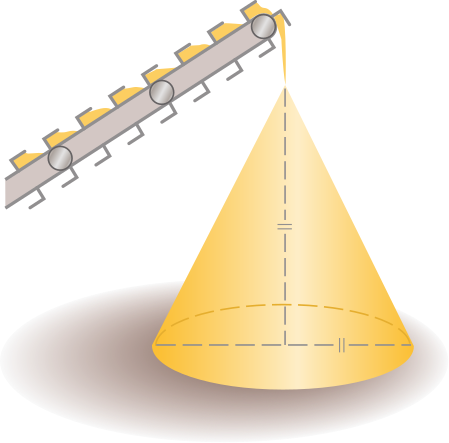
\includegraphics[width=6cm]{./png/3.9.29.png}
    \end{center}

\newpage

\item[3.9.30]
    A swimming pool is $20$ ft wide, $40$ ft long, $3$ ft deep at the shallow end,
    and $9$ ft deep at its deepest point. A cross-section is shown in the figure.
    If the pool is being filled at a rate of $0.8$ ft$^3$/min, how fast is the water level
    rising when the depth at the deepest point is $5$ ft?

    \begin{center}
        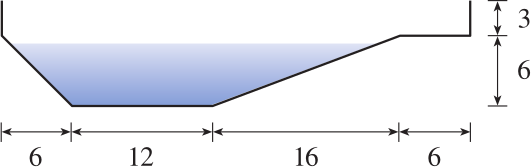
\includegraphics[width=7cm]{./png/3.9.30.png}
    \end{center}

\vspace{6cm}


\item[3.9.44]
    Two carts, $A$ and $B$, are connected by a rope $39$ ft long that passes over a pulley $P$.
    The point $Q$ is on the floor $12$ ft directly beneath $P$ and between the
    carts. Cart $A$ is being pulled away from $Q$ at a speed of $2$ ft/s. How fast is
    cart $B$ moving toward $Q$ at the instant when cart $A$ is $5$ ft from $Q$?

    \begin{center}
        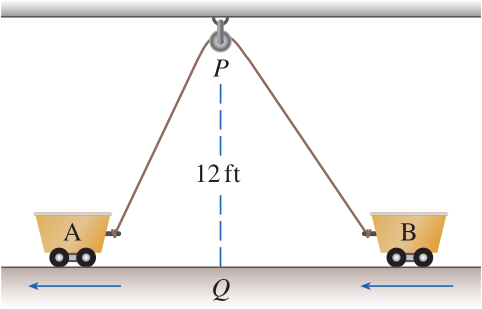
\includegraphics[width=6cm]{./png/3.9.44.png}
    \end{center}

\newpage

\item[3.9.53]
    Suppose that the volume $V$ of a rolling snowball increases so that $\displaystyle \frac{dV}{dt}$ is
    proportional to the surface area of the snowball at time $t$. Show that the radius $r$ increases
    at a constant rate, that is $\displaystyle  \frac{dr}{dt}$ is constant.

\vspace{6cm}

\item[3.10.48]
    When blood flows along a blood vessel, the flux $F$ (the volume of
    blood per unit time that flows past a given point) is proportional
    to the fourth power of the radius $R$ of the blood vessel:
    \[
        F = kR^{4}
    \]
    (This is known as Poiseuilles's Law) A partially clogged artery can be
    expanded by an operation called angioplasty, in which a balloon-tipped
    catheter is inflated inside the artery in order to widen it and restore
    normal blood flow.

    Show that the relative change in $F$ is about four times the relative change
    in $R$. How will a $5$\%  increase in the radius affect the flow of blood?


\newpage

\item[3.10.50]
    In physics textbooks, the period $T$ of a pendulum of length $L$ is
    often given at $T \approx 2 \pi \sqrt{L / g}$, provided that the
    pendulum swings through a relatively small arc. In the course of
    deriving this formula, the equation $a_{T} = -g \sin  \theta  $ for
    the tangential acceleration of the bob of the pendulum is obtained,
    and then $ \sin  \theta   $ is replaced by $ \theta $ with the remark
    that for small angles, $ \theta $(in radians) is very close to
    $ \sin ( \theta  ) $.

    \begin{enumerate}
        \item
            Verify the linear approximation at $0$ for the sine function:
            $\displaystyle  \sin  \theta   \approx \theta $
        \item
            If $ \theta = \pi / 18$(equivalent to $10^{\circ}$) and we
            approximate $\sin  \theta   $ by $ \theta $,
            what is the percentage error?
        \item
            Use a graph to determine the values of $ \theta $ for which $ \sin  \theta  $
            and $ \theta $ differ by less than $2\%$.  What are the values in degrees?
    \end{enumerate}

\vspace{7cm}

\item[3.10.52]
    Suppose that we don't have a formula $g(x)$ but we know that
    $g(2) = -4$ and $g'(x) = \sqrt{x^{2} + 5}$ for all $x$.
    \begin{enumerate}
        \item
            Use a linear approximation to estimate $g(1.95)$ and $g(2.05)$.
        \item
            Are your estimates in part (a) too large or too small? Explain.
    \end{enumerate}

\newpage

\item[4.1.45]
    Find the critical numbers of the function: $f( \theta  ) = 2 \cos ( \theta  ) + \sin^{2} ( \theta  )  $.

\vspace{6cm}

\item[4.1.50]
    A formula for the \textit{derivative} of a function $f$ is given. How many critical
    numbers does $f$ have?
    \[
        f'(x) = \frac{100 \cos^{2}x}{10 + x^{2}} - 1
    \]

\vspace{6cm}

\item[4.1.60]
    Find the absolute maximum/minimum values of $f$ on the given interval.
    \[
        f(x) = \frac{e^{x}}{1 + x^{2}},\ [0, 3]
    \]

\newpage

\item[4.1.63]
    Find the absolute maximum/minimum values of $f$ on the given interval.
    \[
        f(x) = x^{-2} \ln x,\ \left[\frac{1}{2}, 4\right]
    \]

\vspace{6cm}


\item[4.1.66]
    Find the absolute maximum/minimum values of $f$ on the given interval.
    \[
        f(x) = x - 2 \tan^{-1} x,\ [0, 4]
    \]


\end{enumerate}
\end{document}
